% !TEX encoding = UTF-8 Unicode
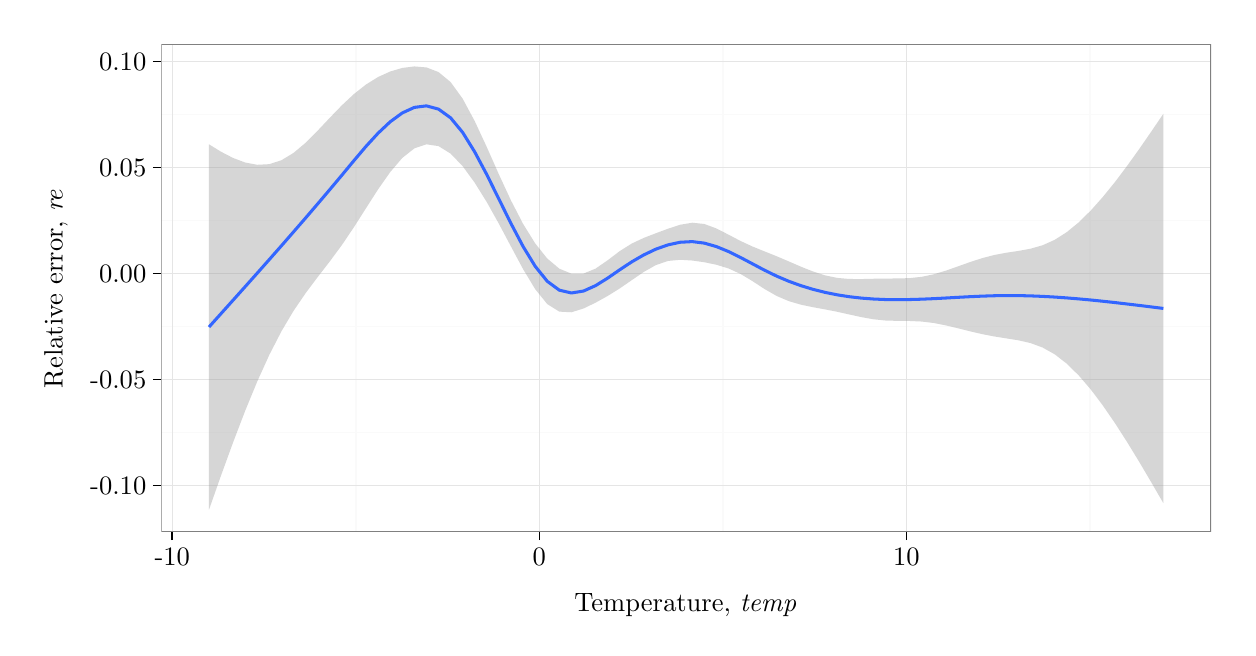
\begin{tikzpicture}[x=1pt,y=1pt]
\definecolor{fillColor}{RGB}{255,255,255}
\path[use as bounding box,fill=fillColor,fill opacity=0.00] (0,0) rectangle (433.62,216.81);
\begin{scope}
\path[clip] (  0.00,  0.00) rectangle (433.62,216.81);
\definecolor{drawColor}{RGB}{255,255,255}
\definecolor{fillColor}{RGB}{255,255,255}

\path[draw=drawColor,line width= 0.6pt,line join=round,line cap=round,fill=fillColor] (  0.00,  0.00) rectangle (433.62,216.81);
\end{scope}
\begin{scope}
\path[clip] ( 48.27, 34.62) rectangle (427.62,210.81);
\definecolor{fillColor}{RGB}{255,255,255}

\path[fill=fillColor] ( 48.27, 34.62) rectangle (427.62,210.81);
\definecolor{drawColor}{gray}{0.98}

\path[draw=drawColor,line width= 0.6pt,line join=round] ( 48.27, 70.57) --
	(427.62, 70.57);

\path[draw=drawColor,line width= 0.6pt,line join=round] ( 48.27,108.88) --
	(427.62,108.88);

\path[draw=drawColor,line width= 0.6pt,line join=round] ( 48.27,147.18) --
	(427.62,147.18);

\path[draw=drawColor,line width= 0.6pt,line join=round] ( 48.27,185.49) --
	(427.62,185.49);

\path[draw=drawColor,line width= 0.6pt,line join=round] (118.57, 34.62) --
	(118.57,210.81);

\path[draw=drawColor,line width= 0.6pt,line join=round] (251.21, 34.62) --
	(251.21,210.81);

\path[draw=drawColor,line width= 0.6pt,line join=round] (383.85, 34.62) --
	(383.85,210.81);
\definecolor{drawColor}{gray}{0.90}

\path[draw=drawColor,line width= 0.2pt,line join=round] ( 48.27, 51.42) --
	(427.62, 51.42);

\path[draw=drawColor,line width= 0.2pt,line join=round] ( 48.27, 89.73) --
	(427.62, 89.73);

\path[draw=drawColor,line width= 0.2pt,line join=round] ( 48.27,128.03) --
	(427.62,128.03);

\path[draw=drawColor,line width= 0.2pt,line join=round] ( 48.27,166.34) --
	(427.62,166.34);

\path[draw=drawColor,line width= 0.2pt,line join=round] ( 48.27,204.64) --
	(427.62,204.64);

\path[draw=drawColor,line width= 0.2pt,line join=round] ( 52.25, 34.62) --
	( 52.25,210.81);

\path[draw=drawColor,line width= 0.2pt,line join=round] (184.89, 34.62) --
	(184.89,210.81);

\path[draw=drawColor,line width= 0.2pt,line join=round] (317.53, 34.62) --
	(317.53,210.81);
\definecolor{fillColor}{RGB}{153,153,153}

\path[fill=fillColor,fill opacity=0.40] ( 65.52,174.65) --
	( 69.88,171.97) --
	( 74.25,169.71) --
	( 78.61,168.07) --
	( 82.98,167.26) --
	( 87.34,167.49) --
	( 91.71,168.91) --
	( 96.07,171.55) --
	(100.44,175.22) --
	(104.80,179.60) --
	(109.17,184.24) --
	(113.54,188.76) --
	(117.90,192.83) --
	(122.27,196.27) --
	(126.63,198.98) --
	(131.00,200.97) --
	(135.36,202.25) --
	(139.73,202.80) --
	(144.09,202.44) --
	(148.46,200.76) --
	(152.82,197.16) --
	(157.19,191.12) --
	(161.55,183.01) --
	(165.92,173.61) --
	(170.28,163.77) --
	(174.65,154.33) --
	(179.01,145.91) --
	(183.38,138.86) --
	(187.75,133.39) --
	(192.11,129.72) --
	(196.48,127.92) --
	(200.84,127.95) --
	(205.21,129.74) --
	(209.57,132.75) --
	(213.94,136.07) --
	(218.30,138.81) --
	(222.67,140.85) --
	(227.03,142.54) --
	(231.40,144.16) --
	(235.76,145.59) --
	(240.13,146.33) --
	(244.49,145.87) --
	(248.86,144.26) --
	(253.23,142.02) --
	(257.59,139.73) --
	(261.96,137.71) --
	(266.32,135.94) --
	(270.69,134.19) --
	(275.05,132.33) --
	(279.42,130.44) --
	(283.78,128.70) --
	(288.15,127.30) --
	(292.51,126.39) --
	(296.88,126.00) --
	(301.24,125.97) --
	(305.61,126.08) --
	(309.97,126.16) --
	(314.34,126.18) --
	(318.71,126.31) --
	(323.07,126.78) --
	(327.44,127.70) --
	(331.80,129.01) --
	(336.17,130.55) --
	(340.53,132.11) --
	(344.90,133.52) --
	(349.26,134.66) --
	(353.63,135.48) --
	(357.99,136.13) --
	(362.36,136.93) --
	(366.72,138.17) --
	(371.09,140.13) --
	(375.45,142.90) --
	(379.82,146.48) --
	(384.19,150.78) --
	(388.55,155.68) --
	(392.92,161.07) --
	(397.28,166.86) --
	(401.65,172.95) --
	(406.01,179.26) --
	(410.38,185.70) --
	(410.38, 44.99) --
	(406.01, 52.53) --
	(401.65, 59.92) --
	(397.28, 67.07) --
	(392.92, 73.87) --
	(388.55, 80.22) --
	(384.19, 86.02) --
	(379.82, 91.12) --
	(375.45, 95.42) --
	(371.09, 98.80) --
	(366.72,101.24) --
	(362.36,102.85) --
	(357.99,103.84) --
	(353.63,104.54) --
	(349.26,105.23) --
	(344.90,106.08) --
	(340.53,107.09) --
	(336.17,108.18) --
	(331.80,109.23) --
	(327.44,110.09) --
	(323.07,110.62) --
	(318.71,110.82) --
	(314.34,110.86) --
	(309.97,110.99) --
	(305.61,111.44) --
	(301.24,112.22) --
	(296.88,113.18) --
	(292.51,114.15) --
	(288.15,115.01) --
	(283.78,115.80) --
	(279.42,116.71) --
	(275.05,117.99) --
	(270.69,119.84) --
	(266.32,122.34) --
	(261.96,125.19) --
	(257.59,127.82) --
	(253.23,129.81) --
	(248.86,131.15) --
	(244.49,132.05) --
	(240.13,132.67) --
	(235.76,132.94) --
	(231.40,132.51) --
	(227.03,131.04) --
	(222.67,128.58) --
	(218.30,125.59) --
	(213.94,122.58) --
	(209.57,119.86) --
	(205.21,117.44) --
	(200.84,115.33) --
	(196.48,113.97) --
	(192.11,114.20) --
	(187.75,116.93) --
	(183.38,122.34) --
	(179.01,129.58) --
	(174.65,137.72) --
	(170.28,145.95) --
	(165.92,153.74) --
	(161.55,160.77) --
	(157.19,166.76) --
	(152.82,171.31) --
	(148.46,174.01) --
	(144.09,174.66) --
	(139.73,173.19) --
	(135.36,169.73) --
	(131.00,164.63) --
	(126.63,158.40) --
	(122.27,151.60) --
	(117.90,144.74) --
	(113.54,138.27) --
	(109.17,132.35) --
	(104.80,126.70) --
	(100.44,120.89) --
	( 96.07,114.48) --
	( 91.71,107.13) --
	( 87.34, 98.64) --
	( 82.98, 89.02) --
	( 78.61, 78.42) --
	( 74.25, 67.02) --
	( 69.88, 55.03) --
	( 65.52, 42.63) --
	cycle;
\definecolor{drawColor}{RGB}{51,102,255}

\path[draw=drawColor,line width= 1.1pt,line join=round] ( 65.52,108.64) --
	( 69.88,113.50) --
	( 74.25,118.37) --
	( 78.61,123.24) --
	( 82.98,128.14) --
	( 87.34,133.06) --
	( 91.71,138.02) --
	( 96.07,143.02) --
	(100.44,148.06) --
	(104.80,153.15) --
	(109.17,158.30) --
	(113.54,163.51) --
	(117.90,168.78) --
	(122.27,173.93) --
	(126.63,178.69) --
	(131.00,182.80) --
	(135.36,185.99) --
	(139.73,188.00) --
	(144.09,188.55) --
	(148.46,187.38) --
	(152.82,184.23) --
	(157.19,178.94) --
	(161.55,171.89) --
	(165.92,163.68) --
	(170.28,154.86) --
	(174.65,146.03) --
	(179.01,137.75) --
	(183.38,130.60) --
	(187.75,125.16) --
	(192.11,121.96) --
	(196.48,120.94) --
	(200.84,121.64) --
	(205.21,123.59) --
	(209.57,126.31) --
	(213.94,129.32) --
	(218.30,132.20) --
	(222.67,134.72) --
	(227.03,136.79) --
	(231.40,138.33) --
	(235.76,139.27) --
	(240.13,139.50) --
	(244.49,138.96) --
	(248.86,137.71) --
	(253.23,135.92) --
	(257.59,133.77) --
	(261.96,131.45) --
	(266.32,129.14) --
	(270.69,127.01) --
	(275.05,125.16) --
	(279.42,123.58) --
	(283.78,122.25) --
	(288.15,121.15) --
	(292.51,120.27) --
	(296.88,119.59) --
	(301.24,119.09) --
	(305.61,118.76) --
	(309.97,118.57) --
	(314.34,118.52) --
	(318.71,118.57) --
	(323.07,118.70) --
	(327.44,118.89) --
	(331.80,119.12) --
	(336.17,119.37) --
	(340.53,119.60) --
	(344.90,119.80) --
	(349.26,119.94) --
	(353.63,120.01) --
	(357.99,119.99) --
	(362.36,119.89) --
	(366.72,119.71) --
	(371.09,119.47) --
	(375.45,119.16) --
	(379.82,118.80) --
	(384.19,118.40) --
	(388.55,117.95) --
	(392.92,117.47) --
	(397.28,116.96) --
	(401.65,116.44) --
	(406.01,115.90) --
	(410.38,115.35);
\definecolor{drawColor}{gray}{0.50}

\path[draw=drawColor,line width= 0.6pt,line join=round,line cap=round] ( 48.27, 34.62) rectangle (427.62,210.81);
\end{scope}
\begin{scope}
\path[clip] (  0.00,  0.00) rectangle (433.62,216.81);
\definecolor{drawColor}{RGB}{0,0,0}

\node[text=drawColor,anchor=base east,inner sep=0pt, outer sep=0pt, scale=  0.96] at ( 42.87, 48.11) {-0.10};

\node[text=drawColor,anchor=base east,inner sep=0pt, outer sep=0pt, scale=  0.96] at ( 42.87, 86.42) {-0.05};

\node[text=drawColor,anchor=base east,inner sep=0pt, outer sep=0pt, scale=  0.96] at ( 42.87,124.72) {0.00};

\node[text=drawColor,anchor=base east,inner sep=0pt, outer sep=0pt, scale=  0.96] at ( 42.87,163.03) {0.05};

\node[text=drawColor,anchor=base east,inner sep=0pt, outer sep=0pt, scale=  0.96] at ( 42.87,201.33) {0.10};
\end{scope}
\begin{scope}
\path[clip] (  0.00,  0.00) rectangle (433.62,216.81);
\definecolor{drawColor}{RGB}{0,0,0}

\path[draw=drawColor,line width= 0.6pt,line join=round] ( 45.27, 51.42) --
	( 48.27, 51.42);

\path[draw=drawColor,line width= 0.6pt,line join=round] ( 45.27, 89.73) --
	( 48.27, 89.73);

\path[draw=drawColor,line width= 0.6pt,line join=round] ( 45.27,128.03) --
	( 48.27,128.03);

\path[draw=drawColor,line width= 0.6pt,line join=round] ( 45.27,166.34) --
	( 48.27,166.34);

\path[draw=drawColor,line width= 0.6pt,line join=round] ( 45.27,204.64) --
	( 48.27,204.64);
\end{scope}
\begin{scope}
\path[clip] (  0.00,  0.00) rectangle (433.62,216.81);
\definecolor{drawColor}{RGB}{0,0,0}

\path[draw=drawColor,line width= 0.6pt,line join=round] ( 52.25, 31.62) --
	( 52.25, 34.62);

\path[draw=drawColor,line width= 0.6pt,line join=round] (184.89, 31.62) --
	(184.89, 34.62);

\path[draw=drawColor,line width= 0.6pt,line join=round] (317.53, 31.62) --
	(317.53, 34.62);
\end{scope}
\begin{scope}
\path[clip] (  0.00,  0.00) rectangle (433.62,216.81);
\definecolor{drawColor}{RGB}{0,0,0}

\node[text=drawColor,anchor=base,inner sep=0pt, outer sep=0pt, scale=  0.96] at ( 52.25, 22.61) {-10};

\node[text=drawColor,anchor=base,inner sep=0pt, outer sep=0pt, scale=  0.96] at (184.89, 22.61) {0};

\node[text=drawColor,anchor=base,inner sep=0pt, outer sep=0pt, scale=  0.96] at (317.53, 22.61) {10};
\end{scope}
\begin{scope}
\path[clip] (  0.00,  0.00) rectangle (433.62,216.81);
\definecolor{drawColor}{RGB}{0,0,0}

\node[text=drawColor,anchor=base,inner sep=0pt, outer sep=0pt, scale=  0.96] at (237.95,  6.00) {Temperature, $\mathit{temp}$};
\end{scope}
\begin{scope}
\path[clip] (  0.00,  0.00) rectangle (433.62,216.81);
\definecolor{drawColor}{RGB}{0,0,0}

\node[text=drawColor,rotate= 90.00,anchor=base,inner sep=0pt, outer sep=0pt, scale=  0.96] at ( 12.61,122.72) {Relative error, $\mathit{re}$};
\end{scope}
\end{tikzpicture}
